%%%%%%%%%%%%%%%%%%%%%%%%%%%%%%%%%%%%%%%%%%%%%%%%%%%%%%%%%%%%%%%%%%%%%%%%%%%%%%%%%%
\begin{frame}[fragile]\frametitle{}
\begin{center}
{\Large Interactive Learning}

{\tiny (Ref: https://rasa.com/docs/rasa/core/interactive-learning/ )}
\end{center}
\end{frame}

%%%%%%%%%%%%%%%%%%%%%%%%%%%%%%%%%%%%%%%%%%%%%%%%%%%%%%%%%%%
 \begin{frame}[fragile]\frametitle{Why Interactive Learning?}
\begin{itemize}
\item Can you teach chatbot, while it is running?
\item Very powerful method
\item Easiest way to fix any mistakes it makes
\item That's advnatage of ML based chatbots, compared to rule-based. If chatbot fails, you can teach it, and then after re-training, it has got corrected.
\end{itemize}
\end{frame}

%%%%%%%%%%%%%%%%%%%%%%%%%%%%%%%%%%%%%%%%%%%%%%%%%%%%%%%%%%%
 \begin{frame}[fragile]\frametitle{Running Interactive Learning}
\begin{lstlisting}
rasa run actions --actions actions&

rasa interactive \
  -m models/20190515-135859.tar.gz \
  --endpoints endpoints.yml
\end{lstlisting}
\end{frame}

%%%%%%%%%%%%%%%%%%%%%%%%%%%%%%%%%%%%%%%%%%%%%%%%%%%%%%%%%%%
 \begin{frame}[fragile]\frametitle{Interactive Learning}
 Rasa will ask you to confirm every prediction made by NLU and Core before proceeding. 
\begin{lstlisting}
Bot loaded. Type a message and press enter (use '/stop' to exit).

? Next user input:  hello

? Is the NLU classification for 'hello' with intent 'hello' correct?  Yes

------
Chat History

 #    Bot                        You
--------------------------------------------
 1    action_listen
--------------------------------------------
 2                                    hello
                         intent: hello 1.00
------

? The bot wants to run 'utter_greet', correct?  (Y/n)
\end{lstlisting}
\end{frame}

%%%%%%%%%%%%%%%%%%%%%%%%%%%%%%%%%%%%%%%%%%%%%%%%%%%%%%%%%%%
 \begin{frame}[fragile]\frametitle{Interactive Learning Example}
 Rasa will ask you to confirm every prediction made by NLU and Core before proceeding. 
\begin{lstlisting}
Bot loaded. Type a message and press enter (use '/stop' to exit).

? Next user input:  hello

? Is the NLU classification for 'hello' with intent 'hello' correct?  Yes

------
Chat History

 #    Bot                        You
--------------------------------------------
 1    action_listen
--------------------------------------------
 2                                    hello
                         intent: hello 1.00
------

? The bot wants to run 'utter_greet', correct?  (Y/n)
\end{lstlisting}
Say `y' if correct. We continue this loop, chatting with the bot, until the bot chooses the wrong action.
\end{frame}

%%%%%%%%%%%%%%%%%%%%%%%%%%%%%%%%%%%%%%%%%%%%%%%%%%%%%%%%%%%
 \begin{frame}[fragile]\frametitle{Providing feedback on errors}
\begin{lstlisting}
------
Chat History

 #    Bot                                           You
--------------------------------------------------------------
 1    action_listen
--------------------------------------------------------------
 2                                            /search_concerts
                                  intent: search_concerts 1.00
--------------------------------------------------------------
 3    action_search_concerts 0.72
      action_listen 0.78
--------------------------------------------------------------
 4                                            /compare_reviews
                                  intent: compare_reviews 1.00


Current slots:
  concerts: None, venues: None

------
? The bot wants to run 'action_show_concert_reviews', correct?  No
\end{lstlisting}
Say `n' because it chose the wrong action, and we get a new prompt asking for the correct one.
\end{frame}

%%%%%%%%%%%%%%%%%%%%%%%%%%%%%%%%%%%%%%%%%%%%%%%%%%%%%%%%%%%
 \begin{frame}[fragile]\frametitle{Providing feedback on errors}
\begin{lstlisting}
? What is the next action of the bot?  (Use arrow keys)
 > 0.53 action_show_venue_reviews
   0.46 action_show_concert_reviews
   0.00 utter_goodbye
   0.00 action_search_concerts
   0.00 utter_greet
   0.00 action_search_venues
   0.00 action_listen
   0.00 utter_youarewelcome
   0.00 utter_default
   0.00 action_default_fallback
   0.00 action_restart
\end{lstlisting}
In this case, the bot should ``action\_show\_concert\_reviews'' (rather than venue reviews!) so we select that action.
\end{frame}

%%%%%%%%%%%%%%%%%%%%%%%%%%%%%%%%%%%%%%%%%%%%%%%%%%%%%%%%%%%
 \begin{frame}[fragile]\frametitle{Visualization of conversations}
\begin{itemize}
\item Chat history can be plotted.
\item At http://localhost:5005/visualization.html as soon as you’ve started interactive learning.
\item To skip the visualization,run \lstinline|rasa interactive --skip-visualization|
\end{itemize}

\begin{center}
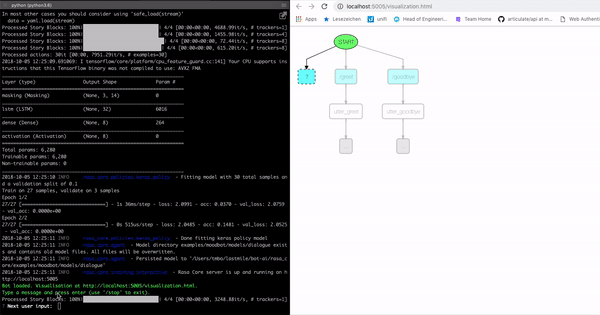
\includegraphics[width=\linewidth]{rasa36}
\end{center}
\end{frame}
